% =============================================================================
% 3 Analyse des bestehenden Erwärmungsprüfstands
% =============================================================================
\section{Analyse des bestehenden Erwärmungsprüfstands}
\label{chap:analyse_pruefstand}

In diesem Kapitel werden der Aufbau, die Funktionsweise und der
gegenwärtige Ablauf der Erwärmungsprüfung untersucht. Ziel ist es, die
für die Stromverteilung maßgebenden elektrischen und mechanischen
Zusammenhänge zu erfassen und damit die Grundlage für die anschließende
Problemanalyse zu schaffen. Aus den dabei festgestellten Schwachstellen
werden im weiteren Verlauf des Kapitels die Anforderungen an das zu
entwickelnde Optimierungskonzept abgeleitet.

Die betrachtete Prüfanordnung besteht aus der regelbaren
Hochstromeinspeisung, einem Anbindefeld sowie einer Prüfkombination aus
Leistungsschalterfeld und MCC-Feld. Das MCC-Feld umfasst zwölf
dreiphasige Abgangseinheiten, die während der Erwärmungsprüfung
gleichzeitig belastet werden. Für die weitere Untersuchung wird eine
Belastungskonfiguration aus sechs A-Modulen mit jeweils
\SI{40}{\ampere}, drei B-Modulen mit jeweils \SI{70}{\ampere} sowie
jeweils einem Abgang mit \SI{250}{\ampere}, \SI{400}{\ampere} und
\SI{630}{\ampere} zugrunde gelegt.

Die Analyse folgt zunächst dem elektrischen Energiepfad vom
Säulenstelltransformator über den Festtransformator und das Anbindefeld
bis zu den MCC-Abgängen und den externen V2A-Lastwiderständen.
Anschließend wird der betriebliche Prüfablauf einschließlich der Strom-
und Temperaturerfassung beschrieben.


% -----------------------------------------------------------------------------
% 3.1 Aufbau und Funktionsweise
% -----------------------------------------------------------------------------
\subsection{Aufbau und Funktionsweise}
\label{sec:aufbau_funktionsweise_pruefstand}

Der bestehende Erwärmungsprüfstand dient der Beaufschlagung von
Nieder\-spannungs-Schalt\-geräte\-kombinationen mit hohen Prüfströmen.
Hierzu wird die aus dem Drehstromnetz bereitgestellte Spannung zunächst
einstellbar gemacht und anschließend auf ein für die Hochstromprüfung
geeignetes niedriges Spannungsniveau transformiert. Die erzeugten
Hochströme werden über massive Kupferschienen und ein Anbindefeld der
zu prüfenden Kombination aus Leistungsschalterfeld und MCC-Feld
zugeführt.

Der funktionale Energiepfad des Prüfstands ist in
Abbildung~\ref{fig:ist_energiepfad} dargestellt. Er verläuft vom
Drehstromnetz über den Säulenstelltransformator, die nachgeschalteten
induktiven Ausgleichselemente und den Festtransformator zur
Hochstromverteilung. Unmittelbar hinter dem Festtransformator werden
die Ströme der drei Außenleiter erfasst. Anschließend wird der
Hochstrom über das Anbindefeld in die Prüfkombination eingespeist.
Innerhalb der Prüfkombination teilt sich der Gesamtstrom auf die zwölf
Abgänge des MCC-Feldes und den über die Kurzschlussbrücke geführten
Stromanteil auf.

\begin{figure}[H]
    \centering
    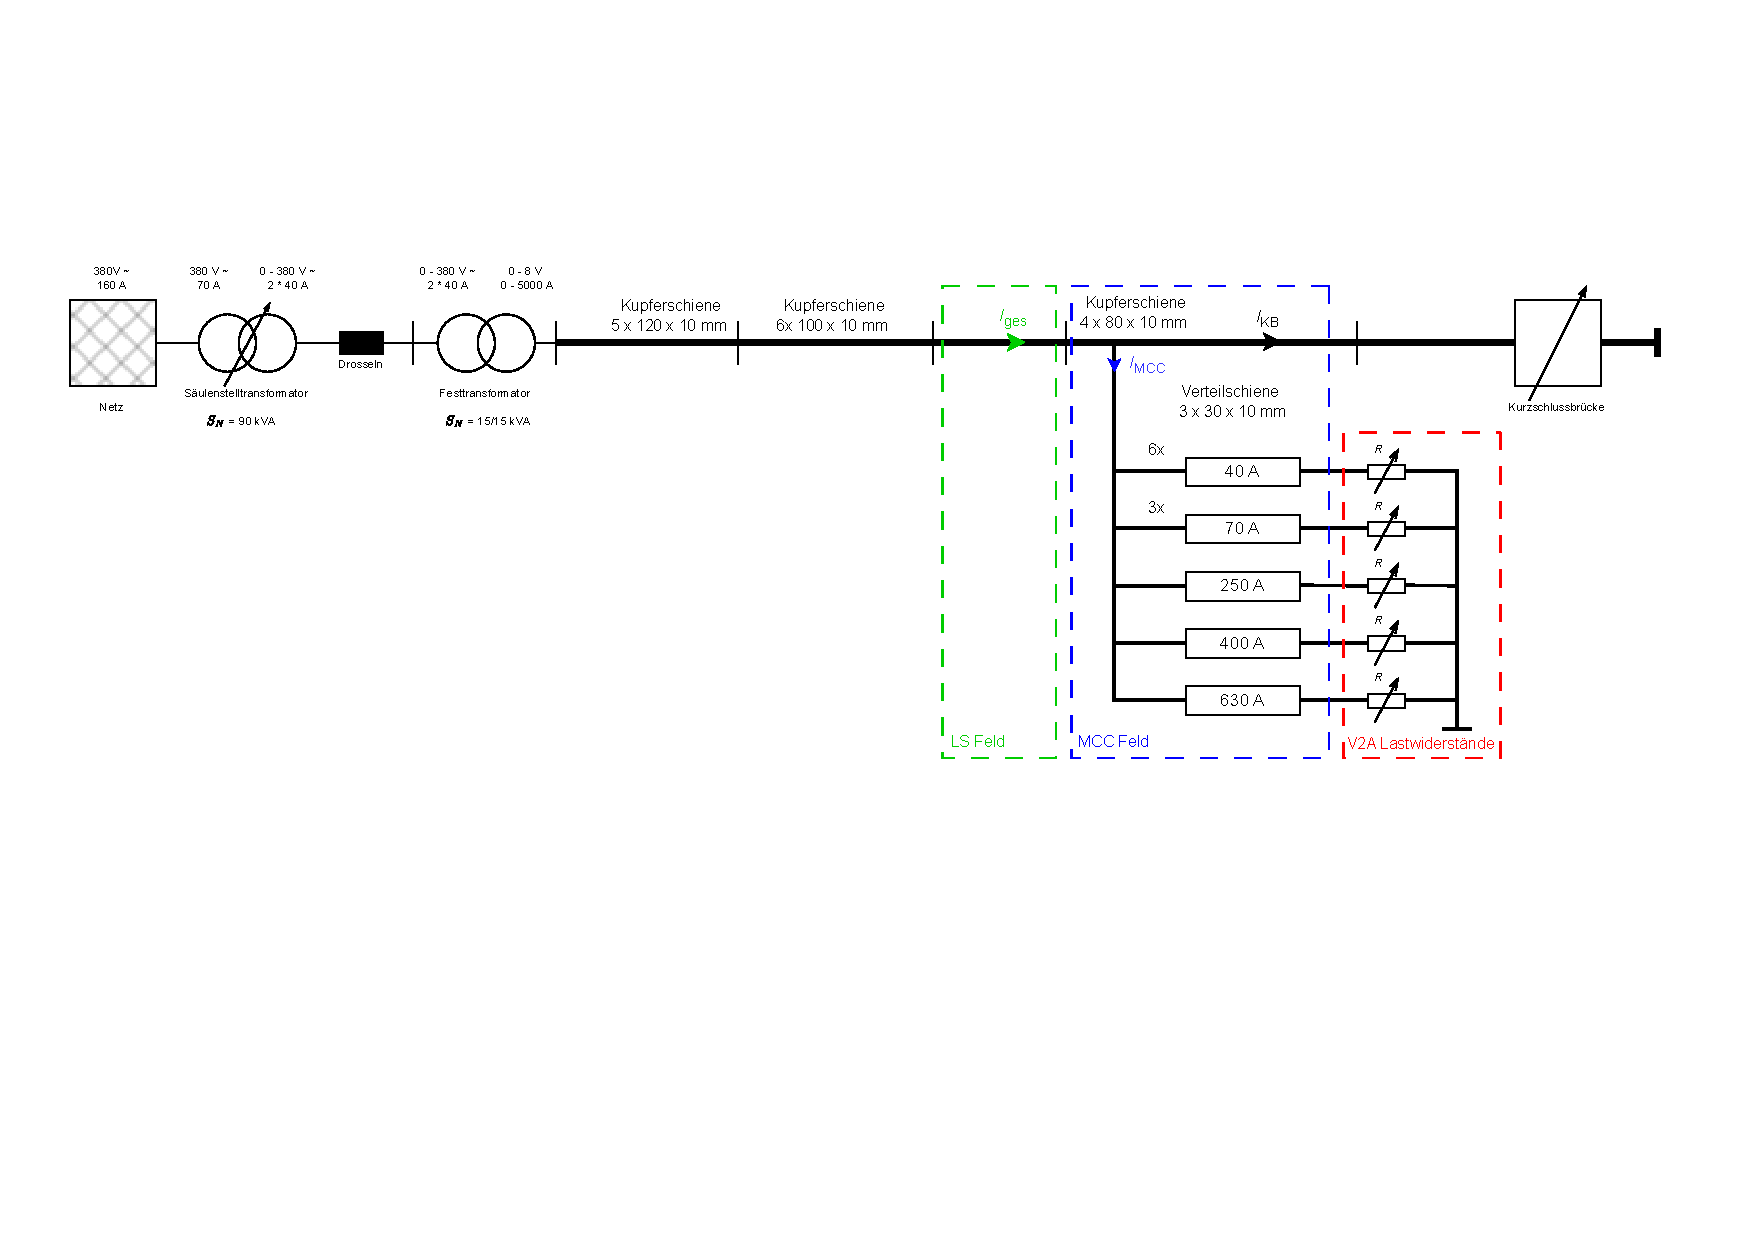
\includegraphics[width=\textwidth]
    {03_Ressourcen/drawio/ESB_Ist-Zustand.pdf}
    \caption{Funktionaler Energiepfad des bestehenden
    Erwärmungsprüfstands mit der betrachteten Belastungskonfiguration
    des MCC-Feldes (eigene Darstellung auf Grundlage der betrieblichen
    Bestandsaufnahme)}
    \label{fig:ist_energiepfad}
\end{figure}


% .............................................................................
% Säulenstelltransformator
% .............................................................................

Die Einspeisung des Prüfstands erfolgt aus dem betrieblichen
\SI{400}{\volt}-Drehstromnetz. Zur Einstellung der dem Festtransformator
zugeführten Spannung wird ein motorisch verstellbarer
Säulenstelltransformator eingesetzt. Das Typenschild des vorhandenen
Betriebsmittels weist eine Nennleistung von
\SI{90}{\kilo\volt\ampere}, eine primäre Nennspannung von
\SI{380}{\volt}, einen primären Nennstrom von \SI{70}{\ampere} und eine
Nennfrequenz von \SI{50}{\hertz} aus. Die von der heutigen
Netzspannung abweichende Spannungsangabe ist auf die historische
Bemessung des im Jahr 1987 gefertigten Transformators zurückzuführen.

Bei einem Säulenstelltransformator wird die Ausgangsspannung durch die
Position der entlang der Wicklung verfahrbaren Stromabnehmer verändert.
Kohlerollen stellen dabei den elektrischen Kontakt zwischen den
Stromabnehmern und den freiliegenden Windungen her. Die Stromabnehmer
werden über eine Antriebswelle, ein Kegelradgetriebe und eine Spindel
in vertikaler Richtung verfahren. Dadurch kann die Ausgangsspannung
auch unter Last kontinuierlich zwischen null und dem vorgesehenen
Endwert eingestellt werden
\parencite[Abschn.~3.2, S.~3]{ruhstrat_betriebsanleitung}.

Der vorhandene Säulenstelltransformator besitzt drei
Wicklungssäulen, die den drei Außenleitern zugeordnet sind. An jeder
Wicklungssäule befinden sich zwei Stromabnehmer, sodass insgesamt sechs
Stromabnehmer vorhanden sind. Die beiden Stromabnehmer einer
Wicklungssäule werden gemeinsam durch einen motorischen Antrieb
verfahren. Insgesamt sind drei motorische Antriebe vorhanden. Die
Abgriffpositionen der drei Außenleiter können daher während des
Betriebs voneinander abweichen.

Tabelle~\ref{tab:ist_saeulenstelltransformator} fasst die für die
weitere Untersuchung relevanten Daten des Säulenstelltransformators
zusammen. Die Angaben wurden dem Typenschild und der betrieblichen
Bestandsaufnahme entnommen.

\begin{table}[H]
    \centering
    \caption{Technische Daten des vorhandenen
    Säulenstelltransformators}
    \label{tab:ist_saeulenstelltransformator}
    \begin{tabular}{
        p{0.44\textwidth}
        p{0.46\textwidth}
    }
        \toprule
        Kenngröße & Wert beziehungsweise Ausführung \\
        \midrule
        Hersteller & Ruhstrat \\
        Baujahr & 1987 \\
        Typ & TKDMT \\
        Nennleistung $S_\mathrm{N}$ &
        \SI{90}{\kilo\volt\ampere} \\
        Primäre Nennspannung $U_\mathrm{1N}$ &
        \SI{380}{\volt} \\
        Primärer Nennstrom $I_\mathrm{1N}$ &
        \SI{70}{\ampere} \\
        Sekundäre Ausgangsspannung &
        je Außenleiter zwei Ausgänge mit
        \SI{0}{\volt} bis \SI{380}{\volt} \\
        Sekundärer Nennstrom &
        je Außenleiter zwei Ausgänge mit
        \SI{40}{\ampere} \\
        Nennfrequenz $f_\mathrm{N}$ &
        \SI{50}{\hertz} \\
        Anzahl der Wicklungssäulen &
        3 \\
        Anzahl der Stromabnehmer &
        6, jeweils zwei je Wicklungssäule \\
        Anzahl der motorischen Antriebe &
        3, jeweils ein Antrieb je Wicklungssäule \\
        \bottomrule
    \end{tabular}
\end{table}

Abbildung~\ref{fig:ist_saeulenstelltransformator} zeigt den geöffneten
Säulenstelltransformator. Erkennbar sind die drei Wicklungssäulen, die
Spindelantriebe und die beidseitig an den Wicklungssäulen angeordneten
Stromabnehmersysteme.

\begin{figure}[H]
    \centering
    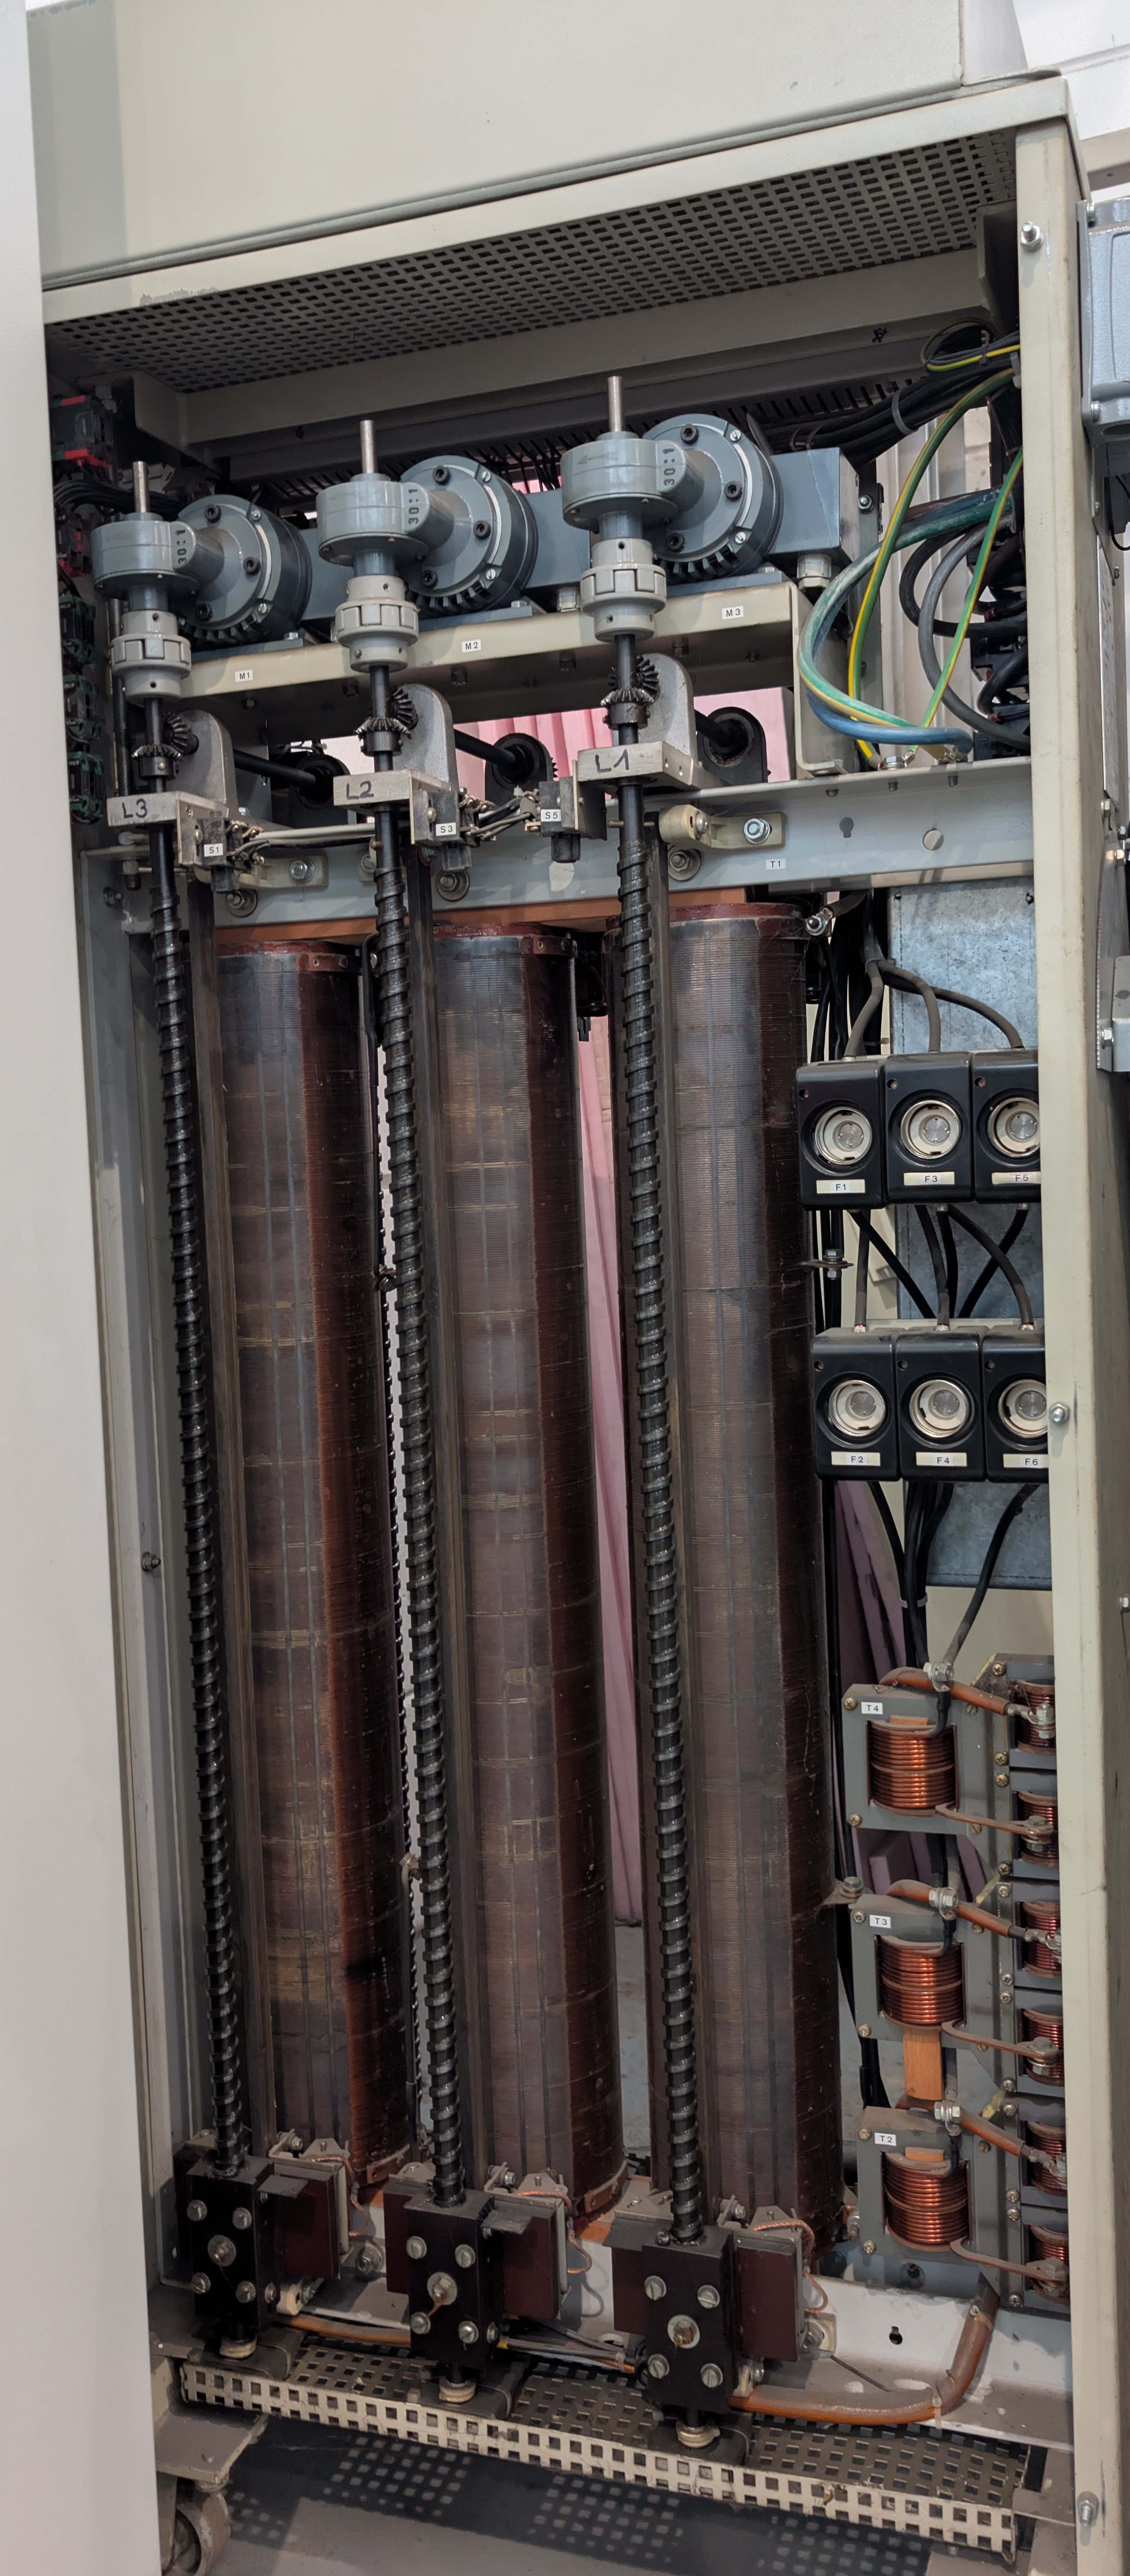
\includegraphics[height=0.50\textheight]
    {03_Ressourcen/pic/stelltrafo.jpg}
    \caption{Geöffneter Säulenstelltransformator mit drei
    Wicklungssäulen, sechs Stromabnehmern und drei motorischen
    Antrieben (eigene Aufnahme)}
    \label{fig:ist_saeulenstelltransformator}
\end{figure}


% .............................................................................
% Induktive Ausgleichselemente
% .............................................................................

Zwischen den Stromabnehmern des Säulenstelltransformators und dem
Festtransformator befinden sich zusätzliche induktive Bauteile, die im
betrieblichen Sprachgebrauch als Drosseln bezeichnet werden. Die
Herstellerunterlagen beschreiben für Säulenstelltransformatoren mit
zwei Stromabnehmern unter anderem beidseitige Schaltungsvarianten sowie
eine galvanisch geteilte Stromschiene mit
Stromausgleichstransformator
\parencite[S.~8--9]{ruhstrat_broschuere_saeulentrafos}. Eine
Ausgleichsfunktion der vorhandenen Bauteile zwischen den beiden
Stromabnehmerpfaden ist daher technisch plausibel.

Eine eindeutige Zuordnung zu einer bestimmten Herstellerschaltung ist
jedoch nicht möglich, da das historische Originalschaltbild des
Transformators nicht mehr vorliegt. Auch der Hersteller konnte die
tatsächliche Verschaltung anhand der verfügbaren Archivunterlagen nicht
rekonstruieren
\parencite[S.~1]{ruhstrat_korrespondenz_2026}. Die Bauteile werden
deshalb im Folgenden neutral als induktive Ausgleichselemente
bezeichnet. Nicht nachgewiesene elektrische Eigenschaften werden ihnen
bei der späteren Modellbildung nicht zugeordnet.

\begin{figure}[H]
    \centering
    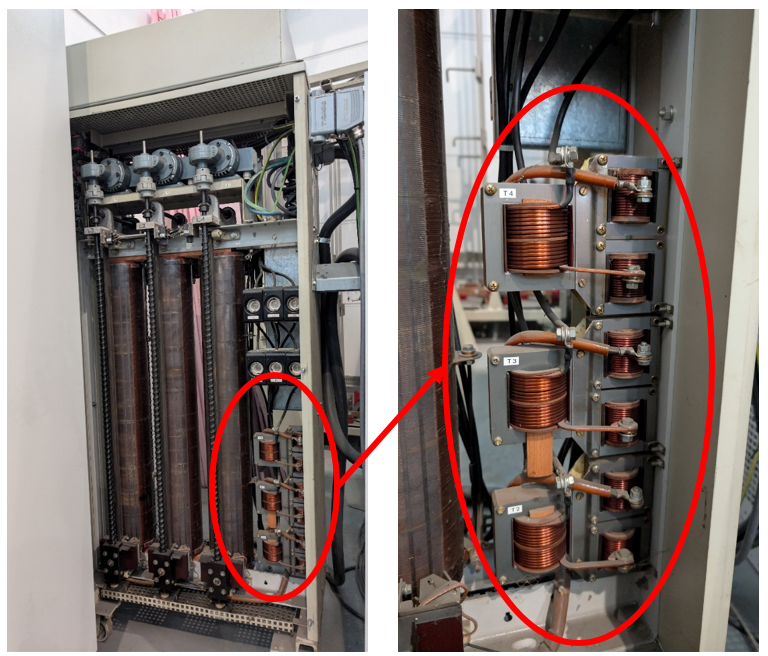
\includegraphics[width=0.92\textwidth]
    {03_Ressourcen/pic/Säulentrafo_Drosseln.png}
    \caption{Anordnung der als Drosseln bezeichneten induktiven
    Ausgleichselemente am Säulenstelltransformator
    (eigene Darstellung und eigene Aufnahmen)}
    \label{fig:ist_ausgleichselemente}
\end{figure}


% .............................................................................
% Festtransformator und zentrale Strommessung
% .............................................................................

Der nachgeschaltete Festtransformator übernimmt die Transformation auf
das für die Erwärmungsprüfung erforderliche Niederspannungsniveau. Das
Typenschild weist primärseitig zwei Wicklungssysteme mit jeweils
\SI{380}{\volt}, \SI{40}{\ampere} und
\SI{15}{\kilo\volt\ampere} aus. Sekundärseitig sind eine
Bemessungsspannung von \SI{6}{\volt} und ein Bemessungsstrom von
\SI{5000}{\ampere} angegeben. Die Kenndaten des Festtransformators sind
in Tabelle~\ref{tab:ist_festtransformator} zusammengefasst.

\begin{table}[H]
    \centering
    \caption{Technische Daten des vorhandenen Festtransformators nach
    Typenschild}
    \label{tab:ist_festtransformator}
    \begin{tabular}{
        p{0.47\textwidth}
        p{0.38\textwidth}
    }
        \toprule
        Kenngröße & Wert \\
        \midrule
        Primäre Nennspannung &
        \SI{380}{\volt} je Wicklungssystem \\
        Primärer Nennstrom &
        \SI{40}{\ampere} je Wicklungssystem \\
        Nennleistung &
        \SI{15}{\kilo\volt\ampere} je Wicklungssystem \\
        Sekundäre Bemessungsspannung &
        \SI{6}{\volt} \\
        Sekundärer Bemessungsstrom &
        \SI{5000}{\ampere} \\
        Nennfrequenz &
        \SI{50}{\hertz} \\
        \bottomrule
    \end{tabular}
\end{table}

Durch die vorgelagerte Einstellung am Säulenstelltransformator kann
sekundärseitig betrieblich ein Spannungsbereich von ungefähr

\begin{equation}
    \SI{0}{\volt}
    \leq
    U_{2,\mathrm{eff}}
    \lesssim
    \SI{8}{\volt}
    \label{eq:ist_spannungsbereich}
\end{equation}

bereitgestellt werden. Die auf dem Typenschild angegebenen
\SI{6}{\volt} kennzeichnen den Bemessungspunkt des Festtransformators.
Der Bereich bis etwa \SI{8}{\volt} beschreibt dagegen den betrieblich
nutzbaren Stellbereich der gesamten Hochstromeinspeisung.

Unmittelbar hinter dem Festtransformator ist für jeden der drei
Außenleiter $L1$, $L2$ und $L3$ ein Stromwandler angeordnet. Nach den
vorliegenden Typenschild- und Anlagenangaben besitzen die
Stromwandler ein Übersetzungsverhältnis von

\begin{equation}
    \frac{I_\mathrm{p}}{I_\mathrm{s}}
    =
    \frac{\SI{5000}{\ampere}}{\SI{5}{\ampere}},
    \label{eq:ist_stromwandler_uebersetzung}
\end{equation}

eine Bemessungsleistung von \SI{10}{\volt\ampere} und die
Genauigkeitsklasse $0{,}2$. Die drei Messwerte werden der zentralen SPS
zugeführt. Diese steuert die motorischen Antriebe des
Säulenstelltransformators so an, dass die übergeordneten Phasenströme
möglichst auf ihren Sollwerten gehalten werden.

Die phasenbezogene Messung und die im Betrieb voneinander abweichenden
mechanischen Stellungen der drei Antriebe sind durch den Anlagenaufbau
belegt. Ohne eine Auswertung des SPS-Programms wird jedoch nicht
unterstellt, dass drei vollständig voneinander unabhängige Regelkreise
implementiert sind.

Die räumliche Anordnung des Festtransformators, der sekundärseitigen
Hochstromverbindungen und der drei nachgeschalteten Stromwandler ist in
Abbildung~\ref{fig:ist_festtransformator} dargestellt.

\begin{figure}[H]
    \centering
    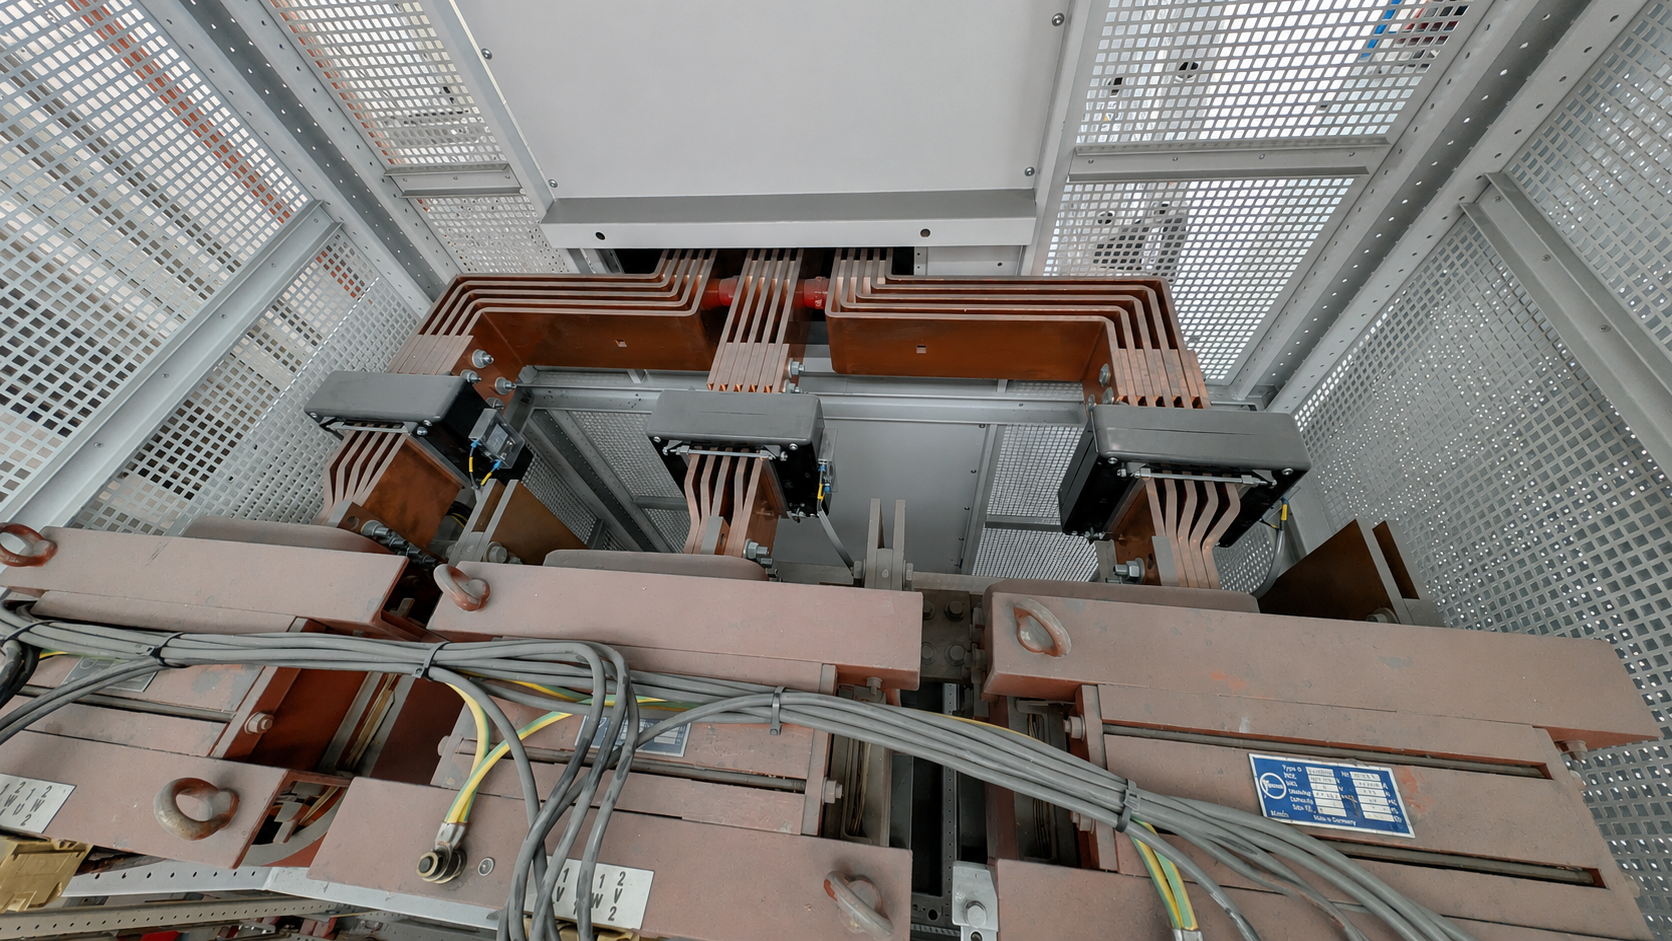
\includegraphics[width=0.95\textwidth]
    {03_Ressourcen/pic/saeulenstelltransformator_festtransformator_strommesswandler.png}
    \caption{Festtransformator mit sekundärseitigen
    Hochstromverbindungen und den drei nachgeschalteten Stromwandlern
    (eigene Aufnahme)}
    \label{fig:ist_festtransformator}
\end{figure}

Regelungstechnisch stellt der Säulenstelltransformator ein
spannungseinstellendes Stellglied dar. Durch die Veränderung seiner
Abgriffpositionen werden die Eingangsspannungen des Festtransformators
und damit dessen sekundärseitige Spannungen verändert. Die
übergeordnete Rückführung erfolgt hingegen anhand der gemessenen
Phasenströme. Der vorgelagerte Anlagenteil bewirkt somit eine
Spannungseinstellung, während die geschlossene Regelungsfunktion als
Stromregelung einzuordnen ist.


% .............................................................................
% Anbindefeld und Prüfkombination
% .............................................................................

Hinter der zentralen Strommessung wird der Hochstrom über das
Anbindefeld zur Prüfkombination geführt. Das Anbindefeld enthält im
Wesentlichen massive Kupferschienen und verschiedene
Anschlussmöglichkeiten für unterschiedliche Prüffeldkonfigurationen.
Es besitzt keine für die vorliegende Untersuchung maßgebende aktive
Schalt- oder Regelfunktion, sondern bildet eine passive
Hochstromschnittstelle zwischen der Einspeisung und der jeweils
angeschlossenen Prüfkombination. Funktional ist es damit mit einem
universell ausgeführten Kuppelfeld vergleichbar.

\begin{figure}[H]
    \centering
    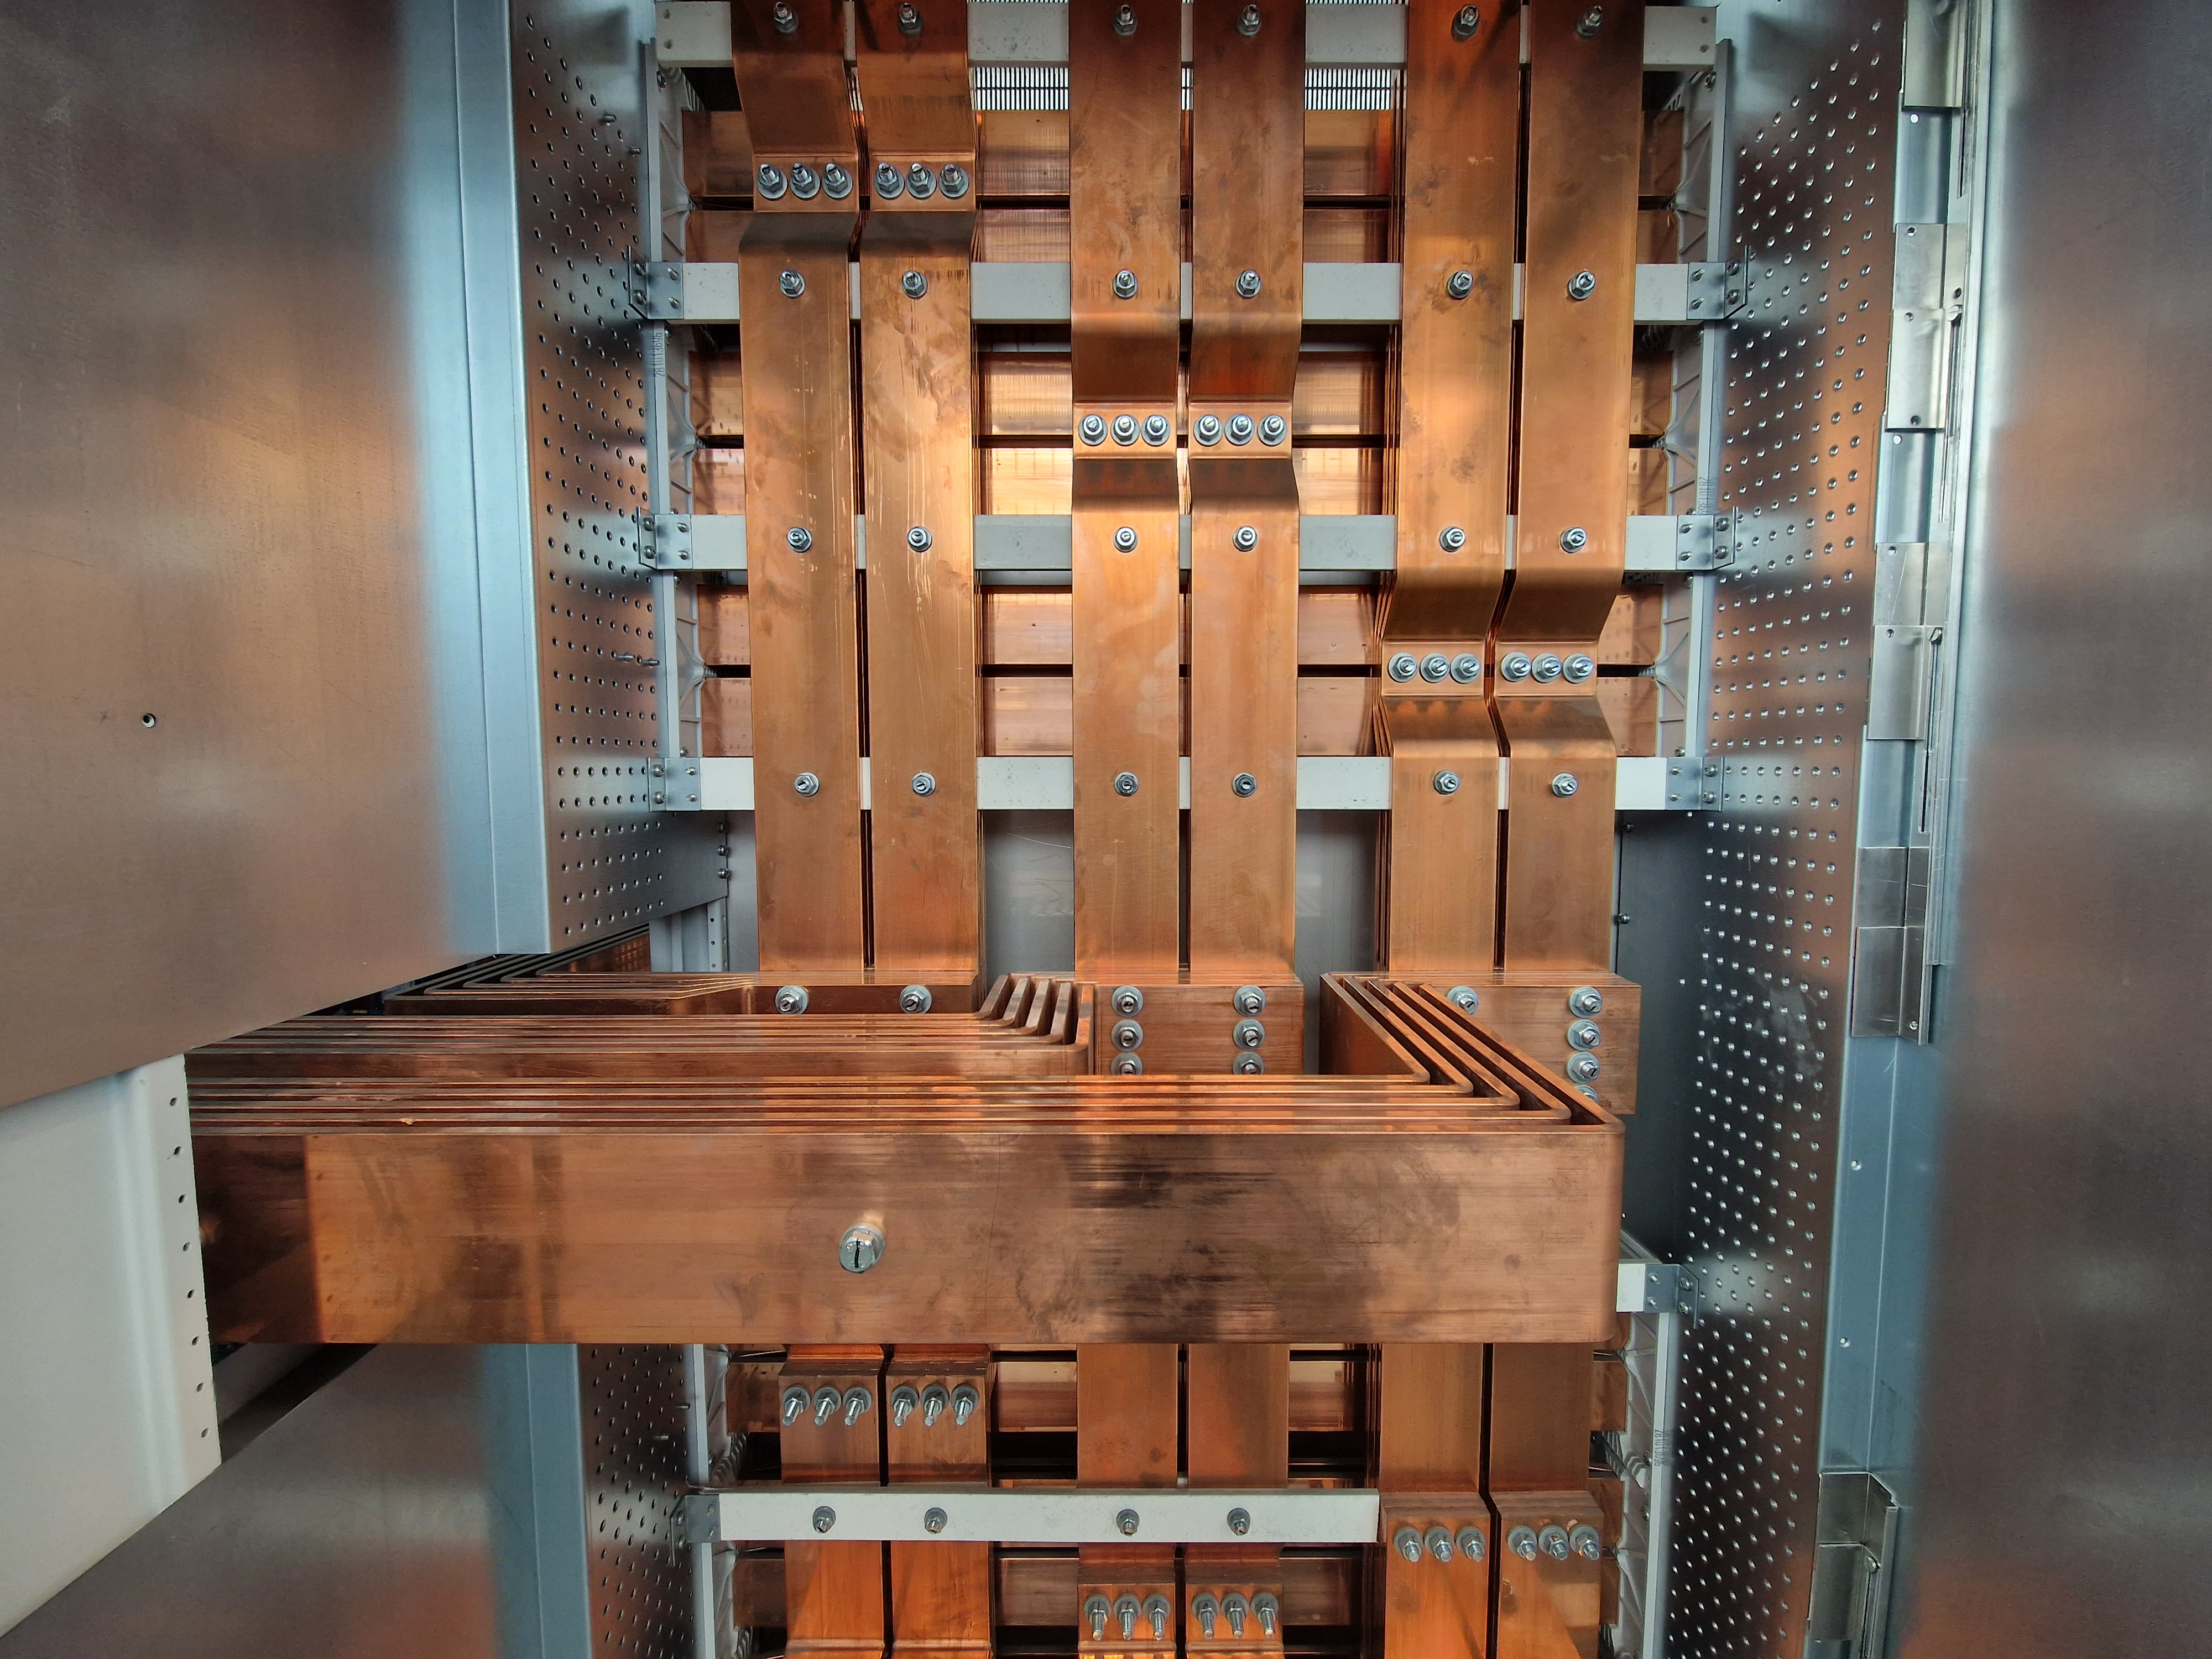
\includegraphics[
        width=0.68\textwidth,
        keepaspectratio
    ]{03_Ressourcen/pic/Anbindefeld.jpg}
    \caption{Kupferschienensystem des als passive
    Hochstromschnittstelle eingesetzten Anbindefeldes
    (eigene Aufnahme)}
    \label{fig:ist_anbindefeld}
\end{figure}

Die betrachtete Prüfkombination besteht aus einem Leistungsschalterfeld
und dem daran angeschlossenen MCC-Feld. Der eingespeiste Gesamtstrom
$I_\mathrm{ges}$ wird über den Leistungsschalter auf das
Hauptsammelschienensystem geführt. Im MCC-Feld teilt sich der Strom auf
die zwölf parallel gespeisten Abgänge und den auf dem
Hauptsammelschienenpfad zur Kurzschlussbrücke weiterfließenden
Stromanteil auf. Für jeden Außenleiter gilt damit die Strombilanz

\begin{equation}
    I_\mathrm{ges}
    =
    I_\mathrm{MCC}
    +
    I_\mathrm{KB},
    \label{eq:ist_strombilanz}
\end{equation}

wobei der Summenstrom des MCC-Feldes durch

\begin{equation}
    I_\mathrm{MCC}
    =
    \sum_{k=1}^{n} I_k,
    \qquad
    n=12
    \label{eq:ist_mcc_summenstrom}
\end{equation}

beschrieben wird. Dabei bezeichnet $I_k$ den Strom des jeweiligen
MCC-Abgangs und $I_\mathrm{KB}$ den über die Kurzschlussbrücke
geführten Strom. Die Bilanz ist für jeden Außenleiter getrennt
anzuwenden. Die Ströme der drei Außenleiter werden nicht miteinander
addiert.

Die für die weitere Untersuchung zugrunde gelegte
Belastungskonfiguration ist in
Tabelle~\ref{tab:mcc_belastungskonfiguration} aufgeführt.

\begin{table}[H]
    \centering
    \caption{Betrachtete Belastungskonfiguration des MCC-Feldes}
    \label{tab:mcc_belastungskonfiguration}
    \begin{tabular}{lccc}
        \toprule
        Modulgruppe &
        Anzahl &
        Strom je Abgang &
        Teilsumme \\
        \midrule
        A-Module &
        6 &
        \SI{40}{\ampere} &
        \SI{240}{\ampere} \\
        B-Module &
        3 &
        \SI{70}{\ampere} &
        \SI{210}{\ampere} \\
        \SI{250}{\ampere}-Modul &
        1 &
        \SI{250}{\ampere} &
        \SI{250}{\ampere} \\
        \SI{400}{\ampere}-Modul &
        1 &
        \SI{400}{\ampere} &
        \SI{400}{\ampere} \\
        \SI{630}{\ampere}-Modul &
        1 &
        \SI{630}{\ampere} &
        \SI{630}{\ampere} \\
        \midrule
        Gesamt &
        12 &
        -- &
        \SI{1730}{\ampere} \\
        \bottomrule
    \end{tabular}
\end{table}

Damit ergibt sich für den Summenstrom des MCC-Feldes je Außenleiter

\begin{equation}
\begin{aligned}
    I_\mathrm{MCC}
    &=
    6 \cdot \SI{40}{\ampere}
    +
    3 \cdot \SI{70}{\ampere}
    +
    \SI{250}{\ampere}
    +
    \SI{400}{\ampere}
    +
    \SI{630}{\ampere}
    \\
    &=
    \SI{1730}{\ampere}.
\end{aligned}
\label{eq:mcc_summenstrom_belastungskonfiguration}
\end{equation}

Der Gesamtstrom des Prüfstands hängt von der jeweils untersuchten
Prüfanordnung ab. Für einen beispielhaften Gesamtstrom von
$I_\mathrm{ges}=\SI{3200}{\ampere}$ ergibt sich aus
Gleichung~\eqref{eq:ist_strombilanz}

\begin{equation}
\begin{aligned}
    I_\mathrm{KB}
    &=
    I_\mathrm{ges}
    -
    I_\mathrm{MCC}
    \\
    &=
    \SI{3200}{\ampere}
    -
    \SI{1730}{\ampere}
    \\
    &=
    \SI{1470}{\ampere}.
\end{aligned}
\label{eq:ist_kurzschlussbruecke_beispiel}
\end{equation}

Dieses Zahlenbeispiel dient ausschließlich der Veranschaulichung der
Stromaufteilung. Der tatsächliche Gesamtstrom und damit auch der Strom
durch die Kurzschlussbrücke ergeben sich aus der jeweils untersuchten
Prüfkombination.

Die Kurzschlussbrücke stellt eine niederimpedante Verbindung der
Hauptstromschienen her. Dadurch kann das Leistungsschalterfeld mit
einem höheren Strom beaufschlagt werden, als über die zwölf Abgänge des
MCC-Feldes geführt wird. Der Strom durch die Kurzschlussbrücke wird
nicht unabhängig eingestellt, sondern ergibt sich nach
Gleichung~\eqref{eq:ist_strombilanz} aus der Differenz zwischen dem
Gesamtstrom und dem Summenstrom des MCC-Feldes.

\begin{figure}[H]
    \centering
    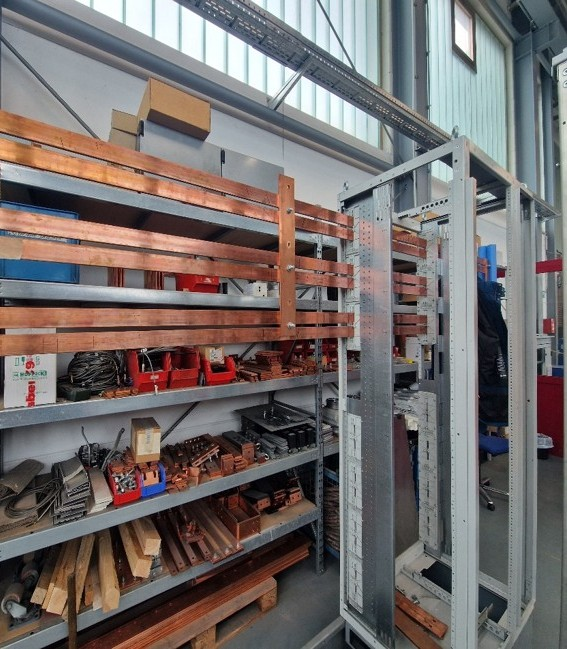
\includegraphics[width=0.72\textwidth]
    {03_Ressourcen/pic/Kurzschlussbrücke.jpg}
    \caption{Kurzschlussbrücke zur niederimpedanten Rückführung des
    nicht über die MCC-Abgänge geführten Stromanteils
    (betriebsinterne Aufnahme)}
    \label{fig:ist_kurzschlussbruecke}
\end{figure}


% .............................................................................
% Aufbau und Strompfad des MCC-Feldes
% .............................................................................

Das MCC-Feld ist funktional in den Geräteraum, den Sammel- und
Verteilschienenbereich sowie den Kabelanschlussraum gegliedert. Im
Geräteraum befinden sich die zwölf dreiphasigen Abgangseinheiten. Der
Kabelanschlussraum nimmt die abgangsseitigen Anschlüsse und die
Verbindungen zu den externen Lastwiderständen auf. Die räumliche
Zuordnung beider Bereiche ist in Abbildung~\ref{fig:ist_mcc_raeume}
dargestellt.

\begin{figure}[H]
    \centering
    \begin{minipage}[c]{0.48\textwidth}
        \centering
        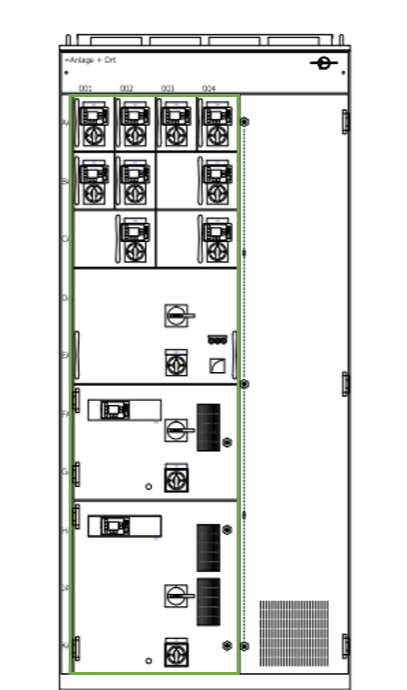
\includegraphics[height=0.47\textheight]
        {03_Ressourcen/pic/MCC_Geräteraum.png}
    \end{minipage}
    \hfill
    \begin{minipage}[c]{0.48\textwidth}
        \centering
        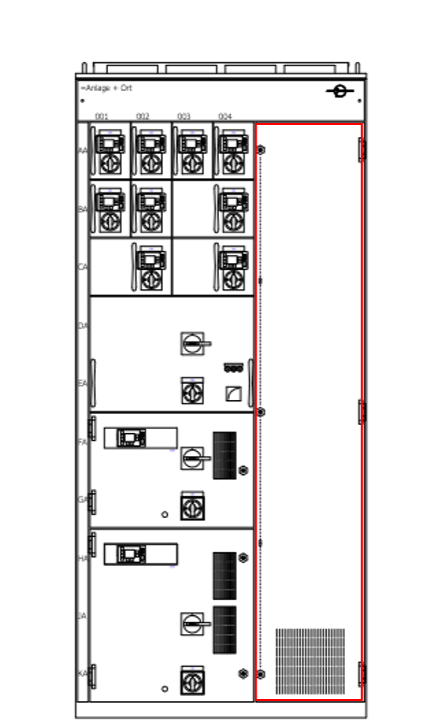
\includegraphics[height=0.47\textheight]
        {03_Ressourcen/pic/MCC_Kabelanschlussraum.png}
    \end{minipage}
    \caption{Kennzeichnung des Geräteraums (links) und des
    Kabelanschlussraums (rechts) am betrachteten MCC-Feld
    (betriebsinterne Darstellungen)}
    \label{fig:ist_mcc_raeume}
\end{figure}

Im rückwärtigen Bereich des Feldes verlaufen die horizontalen
Hauptsammelschienen und die vertikalen Verteilschienen. Das
Hauptsammelschienensystem führt den Gesamtstrom durch das Feld und
weiter zur Kurzschlussbrücke. Von den Hauptsammelschienen zweigen die
vertikalen Verteilschienen ab, über die die parallel angeordneten
MCC-Module gespeist werden. Die Lage der beiden Schienensysteme ist in
Abbildung~\ref{fig:ist_mcc_schienensystem} gekennzeichnet.

\begin{figure}[H]
    \centering
    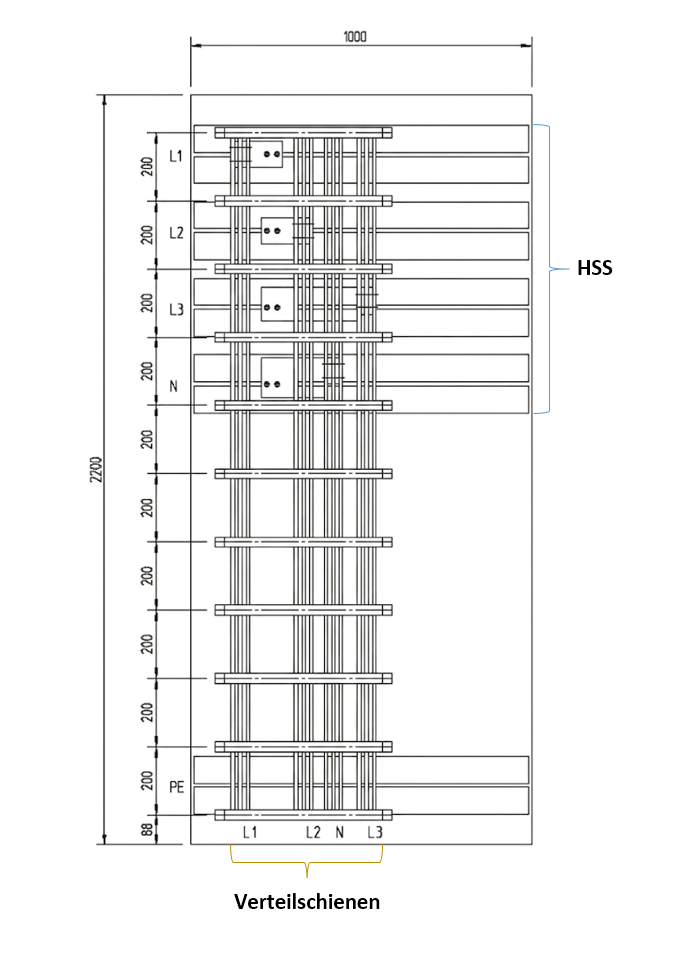
\includegraphics[height=0.72\textheight]
    {03_Ressourcen/pic/Entwurf.png}
    \caption{Anordnung der horizontalen Hauptsammelschienen und der
    vertikalen Verteilschienen im betrachteten MCC-Feld
    (eigene Hervorhebung auf Grundlage der betriebsinternen
    Konstruktionszeichnung)}
    \label{fig:ist_mcc_schienensystem}
\end{figure}

Der Strompfad eines MCC-Abgangs verläuft von der Verteilschiene über
die eingangsseitigen Adapterkontakte in die jeweilige Abgangseinheit.
Innerhalb des Moduls durchfließt der Strom die zu prüfenden Schalt- und
Schutzgeräte. Anschließend wird er über die abgangsseitigen Kontakte in
den Kabelanschlussraum und von dort zu den externen
V2A-Lastwiderständen geführt.

Die betrachtete innere Unterteilung entspricht nach der betrieblichen
Projektdokumentation der Form 4a. Bei dieser Form sind die
Sammelschienen von allen Funktionseinheiten und die Funktionseinheiten
untereinander getrennt. Die Anschlüsse für von außen herangeführte
Leiter liegen im gleichen Abteil wie die zugeordnete Funktionseinheit
\parencite[Tab.~104, S.~43]{din_en_61439_2}.


% .............................................................................
% V2A-Lastwiderstände
% .............................................................................

Die einzelnen MCC-Abgänge werden über verstellbare Lastwiderstände aus
nichtrostendem Stahl belastet. Für jeden Phasenpfad sind zwei räumlich
parallel angeordnete Flachschienen oder L-Schienen vorhanden. Die Bezeichnung
``parallel angeordnet'' beschreibt dabei ausschließlich die
geometrische Anordnung. Elektrisch bilden die beiden Schienen über
eine verschiebbare Brücke einen zusammenhängenden Strompfad.

Eine Schiene ist mit dem Ausgang des MCC-Moduls verbunden, während die
zweite Schiene zum gemeinsamen Sternpunkt führt. Die verschiebbare
Brücke verbindet beide Schienen miteinander. Der Strom fließt zunächst
über die erste Schiene bis zur Position der Brücke und anschließend
über die zweite Schiene zum Sternpunkt. Durch das Verschieben der
Brücke wird die wirksame Leiterlänge und damit der elektrische
Widerstand des Lastpfads verändert.

\begin{figure}[H]
    \centering
    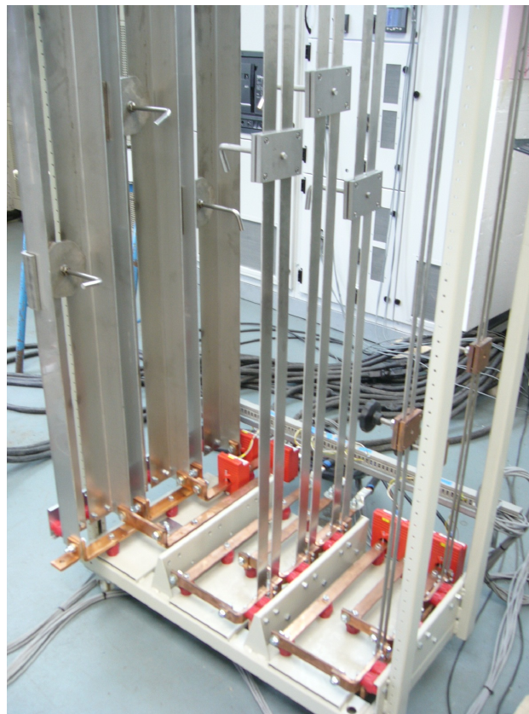
\includegraphics[height=0.68\textheight]
    {03_Ressourcen/pic/Widerstandswagen.png}
    \caption{Widerstandswagen mit paarweise angeordneten
    V2A-Flachschienen und verschiebbaren Brücken zur Einstellung der
    wirksamen Leiterlänge (betriebsinterne Aufnahme)}
    \label{fig:ist_v2a_widerstandswagen}
\end{figure}

Der elektrische Widerstand eines Lastpfads $k$ kann zunächst
näherungsweise durch

\begin{equation}
    R_{\mathrm{V2A},k}
    =
    \rho_\mathrm{V2A}
    \frac{l_{\mathrm{eff},k}}{A_k}
    \label{eq:ist_v2a_widerstand}
\end{equation}

beschrieben werden. Dabei bezeichnet $\rho_\mathrm{V2A}$ den
spezifischen elektrischen Widerstand des verwendeten Werkstoffs,
$A_k$ den Leiterquerschnitt und $l_{\mathrm{eff},k}$ die durch die
Brückenposition bestimmte wirksame Leiterlänge. Der Gesamtwiderstand
eines Abgangspfads setzt sich darüber hinaus aus den Widerständen des
MCC-Moduls, der Kontakte, der Verbindungen und der Zuleitungen
zusammen:

\begin{equation}
    R_{\mathrm{ges},k}
    =
    R_{\mathrm{V2A},k}
    +
    R_{\mathrm{Modul},k}
    +
    R_{\mathrm{Kontakt},k}
    +
    R_{\mathrm{Leitung},k}.
    \label{eq:ist_gesamtwiderstand_abgang}
\end{equation}

Für eine vorgegebene Abgangsspannung $U_k$ ergibt sich der Modulstrom
näherungsweise zu

\begin{equation}
    I_k
    =
    \frac{U_k}{R_{\mathrm{ges},k}}.
    \label{eq:ist_modulstrom}
\end{equation}

Eine Vergrößerung der wirksamen Leiterlänge erhöht den Widerstand und
verringert den zugehörigen Modulstrom. Eine Verkürzung der wirksamen
Leiterlänge bewirkt den entgegengesetzten Effekt. Der Modulstrom wird
im bestehenden Prüfaufbau daher durch manuelles Verschieben der Brücke
eingestellt.


% .............................................................................
% Regelungstechnische Einordnung
% .............................................................................

Die drei unmittelbar hinter dem Festtransformator angeordneten
Stromwandler erfassen die übergeordneten Phasenströme. Diese Messwerte
werden zur motorischen Nachführung des Säulenstelltransformators
verwendet. Die einzelnen Modulströme werden während der Prüfung
ebenfalls phasenweise erfasst, wirken im bestehenden Aufbau jedoch
nicht jeweils auf ein eigenes automatisches Stellglied zurück. Ihre
Korrektur erfolgt durch manuelles Verstellen der zugeordneten
V2A-Lastwiderstände.

Der Ist-Zustand kombiniert damit eine automatische Nachführung der
übergeordneten Phasenströme mit einer manuellen Einstellung der zwölf
Modulströme. Die drei Abgriffpositionen des
Säulenstelltransformators beeinflussen über die bereitgestellten
Spannungen sowohl den Strom durch die Kurzschlussbrücke als auch die
zwölf Modulströme. Gleichzeitig wirken sich Änderungen einzelner
Lastwiderstände auf die Belastung der gemeinsamen Einspeisung aus.

Aufgrund der gemeinsam genutzten Spannungsquelle, der Haupt- und
Verteilschienen sowie der Vielzahl an Teilströmen ist der Prüfstand
regelungstechnisch als gekoppeltes Mehrgrößensystem zu betrachten.
Eine Änderung des Lastwiderstands eines Abgangs beeinflusst zunächst
dessen Modulstrom, verändert gleichzeitig aber auch den Gesamtstrom und
kann dadurch eine Reaktion der übergeordneten Stromregelung
hervorrufen. Die daraus entstehenden Wechselwirkungen werden in
Abschnitt~\ref{sec:problemanalyse_ist} untersucht.

% -----------------------------------------------------------------------------
% 3.2 Derzeitige Durchführung der Erwärmungsprüfung
% -----------------------------------------------------------------------------
\subsection{Derzeitige Durchführung der Erwärmungsprüfung}
\label{sec:durchfuehrung_ist}

Vor Beginn der Erwärmungsprüfung wird die zu untersuchende Kombination
aus Leistungsschalterfeld und MCC-Feld entsprechend dem Prüfauftrag
aufgebaut. Die zwölf dreiphasigen Abgangseinheiten werden in das
MCC-Feld eingesetzt und im Kabelanschlussraum mit den zugeordneten
V2A-Widerstandswagen verbunden. Der durch das Leistungsschalterfeld
geführte Strompfad wird über die Kurzschlussbrücke geschlossen.
Anschließend werden die Hochstromverbindungen, die Zuordnung der
Messkanäle und die Funktionsfähigkeit der erforderlichen
Schutzeinrichtungen kontrolliert.

Zur Erfassung der Erwärmung werden Pt100-Widerstandsthermometer an den
für die Bewertung maßgebenden Bauteilen und Verbindungsstellen
angebracht. Hierzu zählen insbesondere stromführende Verbindungen,
Anschlussstellen, Schaltgeräte und weitere thermisch relevante
Komponenten der zu prüfenden Schaltgerätekombination. Die
Temperaturmesswerte werden von der vorhandenen Messtechnik erfasst und
gemeinsam mit den Strommesswerten in der speicherprogrammierbaren
Steuerung verarbeitet. Die Anzeige und zeitliche Aufzeichnung der
Messwerte erfolgt über das Prozessvisualisierungssystem WinCC.

Neben den drei übergeordneten Phasenströmen unmittelbar hinter dem
Festtransformator werden die Ströme der einzelnen MCC-Abgänge
phasenbezogen erfasst. Damit stehen für jede der zwölf
Abgangseinheiten jeweils Messwerte für \(L1\), \(L2\) und \(L3\) zur
Verfügung. Die wesentlichen Messgrößen und ihre Funktionen im
Prüfablauf sind in
Tabelle~\ref{tab:ist_messgroessen_pruefablauf}
zusammengefasst.

\begin{table}[H]
    \centering
    \caption{Wesentliche Messgrößen der bestehenden Erwärmungsprüfung}
    \label{tab:ist_messgroessen_pruefablauf}
    \begin{tabular}{
        p{0.23\textwidth}
        p{0.32\textwidth}
        p{0.34\textwidth}
    }
        \toprule
        Messgröße &
        Erfassung &
        Funktion im Prüfablauf \\
        \midrule

        Übergeordnete Phasenströme &
        Je ein Stromwandler für \(L1\), \(L2\) und \(L3\) unmittelbar
        hinter dem Festtransformator &
        Rückführung der Istwerte für die zentrale Stromregelung \\

        \addlinespace

        Modulströme &
        Phasenbezogene Strommessung an jedem der zwölf
        V2A-Lastzweige &
        Einstellung und Überwachung der vorgegebenen Ströme der
        einzelnen MCC-Abgänge \\

        \addlinespace

        Temperaturen &
        Pt100-Widerstandsthermometer an den festgelegten
        Messstellen &
        Aufzeichnung des Erwärmungsverlaufs und Beurteilung des
        thermischen Beharrungszustands \\

        \bottomrule
    \end{tabular}
\end{table}

Nach Abschluss der vorbereitenden Kontrollen wird die Prüfanordnung
eingeschaltet. Der übergeordnete Prüfstrom wird anschließend
schrittweise auf den für die jeweilige Prüfung vorgesehenen Sollwert
erhöht. Die SPS verarbeitet hierzu die hinter dem Festtransformator
gemessenen Phasenströme und steuert die motorischen Antriebe des
Säulenstelltransformators an. Durch das Verfahren der Stromabnehmer
ändert sich die dem Festtransformator zugeführte Spannung und damit
der auf dessen Sekundärseite bereitgestellte Hochstrom.

Der Säulenstelltransformator wirkt innerhalb dieser Regelung als
spannungseinstellendes Stellglied. Die geregelten Größen sind jedoch
die gemessenen Phasenströme der Hochstromeinspeisung. Die Stellungen
der drei motorischen Antriebe können im Betrieb voneinander abweichen.
Da die genaue Struktur und Parametrierung der SPS-Regelung nicht
Gegenstand dieser Arbeit ist, wird daraus keine vollständige
Unabhängigkeit dreier einzelner Phasenregelkreise abgeleitet.

Nachdem der übergeordnete Prüfstrom annähernd erreicht ist, werden die
Ströme der zwölf MCC-Abgänge eingestellt. Hierzu verschiebt das
Prüfpersonal die Brücken der zugehörigen V2A-Widerstände und verändert
dadurch deren wirksame Leiterlänge. Die Einstellung kann während der
Bestromung vorgenommen werden, da auf der Sekundärseite des
Festtransformators eine Spannung im Bereich bis ungefähr
\SI{8}{\volt} anliegt.

Für die betrachtete Belastungskonfiguration werden sechs A-Module auf
jeweils \SI{40}{\ampere}, drei B-Module auf jeweils
\SI{70}{\ampere} sowie die drei weiteren Abgangseinheiten auf
\SI{250}{\ampere}, \SI{400}{\ampere} und
\SI{630}{\ampere} eingestellt. Der daraus resultierende Strom des
MCC-Feldes beträgt nach
Gleichung~\eqref{eq:mcc_summenstrom_belastungskonfiguration}
\SI{1730}{\ampere} je Außenleiter.

Die Einstellung der Modulströme erfolgt iterativ. Wird die Position
einer V2A-Brücke verändert, ändern sich der Widerstand und damit der
Strom des betreffenden Abgangs unmittelbar. Gleichzeitig verändert
sich die Belastung der gemeinsamen Hochstromeinspeisung. Die zentrale
Stromregelung kann darauf mit einer Verstellung des
Säulenstelltransformators reagieren, wodurch sich die an den parallel
angeschlossenen MCC-Abgängen anliegende Spannung ebenfalls verändert.
Eine Korrektur eines einzelnen Modulstroms kann deshalb auch die
bereits eingestellten Ströme anderer Abgänge beeinflussen. Nach einer
Verstellung müssen die übrigen Modulströme erneut kontrolliert und
gegebenenfalls nachgestellt werden.

Nach Abschluss der anfänglichen Einstellung beginnt die eigentliche
Erwärmungsphase. Die Abgangseinheiten, die Schienenverbindungen, das
Leistungsschalterfeld und die angeschlossenen Lastwiderstände werden
über mehrere Stunden mit den vorgesehenen Prüfströmen belastet.
Während dieser Zeit werden die Temperaturen, die übergeordneten
Phasenströme und die phasenbezogenen Modulströme fortlaufend erfasst
und in WinCC zeitlich aufgezeichnet.

Die zentrale Stromregelung führt die übergeordneten Phasenströme
während der Erwärmungsprüfung nach. Für die zwölf Modulströme besteht
im Ist-Zustand dagegen keine jeweils zugeordnete automatische
Nachführung. Verändern sich die Widerstände der einzelnen Lastzweige
infolge ihrer Erwärmung, können die zugehörigen Modulströme von ihren
eingestellten Sollwerten abweichen. Diese Abweichungen müssen vom
Prüfpersonal erkannt und durch erneutes Verschieben der jeweiligen
V2A-Brücken manuell korrigiert werden.

Aufgrund der elektrischen Kopplung über die gemeinsame Einspeisung ist
nach einer solchen Korrektur nicht nur der verstellte Abgang zu
kontrollieren. Vielmehr müssen die Stromwerte sämtlicher Abgänge
erneut betrachtet werden. Dieser Vorgang kann sich während einer
Erwärmungsprüfung mehrfach wiederholen und führt zu einem erhöhten
Bedien- und Überwachungsaufwand.

Die Belastung wird fortgeführt, bis sich ein thermischer
Beharrungszustand eingestellt hat. Nach DIN EN IEC 61439-1 gilt dieser
Zustand als erreicht, wenn die Änderung der Temperaturerhöhung an
sämtlichen betrachteten Messstellen höchstens
\SI{1}{\kelvin\per\hour} beträgt
\parencite[Abschn.~10.10.2.3.1]{din_en_61439_1}.
Die in WinCC aufgezeichneten Temperaturverläufe stellen die
erforderliche Datengrundlage zur Beurteilung dieses Kriteriums bereit.
Eine vollständig automatische Bewertung des Beharrungszustands durch
WinCC wird hierbei nicht vorausgesetzt.

Nach Erreichen des thermischen Beharrungszustands werden die
maßgebenden Endwerte der Temperaturen und Ströme dokumentiert und mit
den für die Prüfung geltenden Bewertungskriterien verglichen.
Anschließend wird der Prüfstrom kontrolliert zurückgenommen und die
Prüfanordnung abgeschaltet.

Die wiederholte manuelle Nachstellung der Modulströme sowie deren
gegenseitige Beeinflussung über die gemeinsame Hochstromeinspeisung
bilden den Ausgangspunkt für die nachfolgende Analyse der bestehenden
Problematik.

% -----------------------------------------------------------------------------
% 3.3 Analyse der bestehenden Problematik
% -----------------------------------------------------------------------------
\subsection{Analyse der bestehenden Problematik}
\label{sec:analyse_problematik}

Die zentrale Stromregelung des bestehenden Prüfstands kann den
übergeordneten Prüfstrom jeder Phase nachführen. Für die zwölf
Modulströme des MCC-Feldes besteht dagegen keine individuelle
automatische Nachführung. Diese Ströme werden zwar phasenbezogen
gemessen, ihre Einstellung erfolgt jedoch ausschließlich durch das
manuelle Verstellen der zugehörigen V2A-Widerstände. Die wesentliche
Schwachstelle liegt daher nicht in der grundsätzlichen Bereitstellung
des Hochstroms, sondern in dessen Verteilung auf die einzelnen
MCC-Abgänge.

Die nachfolgende Betrachtung erfolgt stellvertretend für eine Phase.
Da sämtliche Abgangseinheiten dreiphasig ausgeführt sind, treten die
beschriebenen Zusammenhänge grundsätzlich in den Außenleitern
\(L1\), \(L2\) und \(L3\) auf. Auf einen zusätzlichen Phasenindex wird
zur besseren Lesbarkeit verzichtet. Der Index \(k\) kennzeichnet einen
der zwölf parallel gespeisten MCC-Abgänge.

Die in den V2A-Widerständen umgesetzte elektrische Verlustleistung
beträgt nach Gleichung~\eqref{eq:elektrische_verlustleistung}

\begin{equation}
    P_{\mathrm{V2A},k}
    =
    I_k^2 R_{\mathrm{V2A},k}.
    \label{eq:ist_verlustleistung_v2a}
\end{equation}

Die Verlustleistung erwärmt die Widerstandsschienen. Aufgrund des
positiven Temperaturkoeffizienten des eingesetzten nichtrostenden
Stahls steigt deren elektrischer Widerstand mit zunehmender
Temperatur. Ausgehend von
Gleichung~\eqref{eq:widerstand_temperatur} gilt für den Abgang \(k\)

\begin{equation}
    R_{\mathrm{V2A},k}(\vartheta_k)
    =
    R_{\mathrm{V2A},20,k}
    \left[
        1
        +
        \alpha_{20}
        \left(
            \vartheta_k-\SI{20}{\degreeCelsius}
        \right)
    \right].
    \label{eq:ist_v2a_temperaturabhaengigkeit}
\end{equation}

Dabei bezeichnet \(R_{\mathrm{V2A},20,k}\) den Widerstand des
betreffenden V2A-Lastpfads bei \SI{20}{\degreeCelsius},
\(\alpha_{20}\) den elektrischen Temperaturkoeffizienten und
\(\vartheta_k\) die aktuelle Temperatur der Widerstandsschienen.

Der Gesamtwiderstand eines Abgangs setzt sich aus dem
temperaturabhängigen V2A-Widerstand und den weiteren Widerständen des
Strompfads zusammen. Die Leitungs-, Kontakt- und Modulwiderstände
werden für die qualitative Betrachtung zu
\(R_{\mathrm{rest},k}\) zusammengefasst:

\begin{equation}
    R_{\mathrm{ges},k}(\vartheta_k)
    =
    R_{\mathrm{rest},k}
    +
    R_{\mathrm{V2A},k}(\vartheta_k).
    \label{eq:ist_gesamtwiderstand_temperatur}
\end{equation}

Für den Strom des Abgangs folgt damit

\begin{equation}
    I_k(\vartheta_k)
    =
    \frac{U_k}
    {R_{\mathrm{rest},k}
    +
    R_{\mathrm{V2A},k}(\vartheta_k)}.
    \label{eq:ist_modulstrom_temperatur}
\end{equation}

Bei einer zunächst als konstant betrachteten Zweigspannung führt der
temperaturbedingte Widerstandsanstieg unmittelbar zu einer Abnahme des
Modulstroms:

\begin{equation}
    \vartheta_k \uparrow
    \quad\Longrightarrow\quad
    R_{\mathrm{V2A},k} \uparrow
    \quad\Longrightarrow\quad
    I_k \downarrow.
    \label{eq:ist_kausalkette_stromdrift}
\end{equation}

Dieser Vorgang wird im weiteren Verlauf der Arbeit als thermisch
bedingter Stromdrift bezeichnet. Die Annahme einer konstanten
Zweigspannung dient an dieser Stelle lediglich zur Darstellung des
grundlegenden Wirkzusammenhangs. Im realen Prüfstand kann die zentrale
Stromregelung die gemeinsame Einspeisespannung verändern. Da diese
Spannungsänderung jedoch auf sämtliche parallel angeschlossenen
Strompfade wirkt, ist damit keine selektive Korrektur eines einzelnen
Modulstroms möglich.

Der thermisch bedingte Stromdrift tritt nicht bei allen Abgängen in
gleicher Stärke auf. Die Abgänge unterscheiden sich hinsichtlich
ihrer Prüfströme, der eingesetzten Widerstandsquerschnitte, der
eingestellten wirksamen Leiterlängen sowie ihrer elektrischen und
thermischen Randbedingungen. Wegen der quadratischen Abhängigkeit der
Verlustleistung vom Strom werden die Lastzweige unterschiedlich stark
thermisch beansprucht. Daraus ergeben sich voneinander abweichende
Temperatur- und Widerstandsverläufe.

Der von der zentralen Anlagenregelung erfasste Phasenstrom setzt sich
aus dem Strom über die Kurzschlussbrücke und den zwölf Modulströmen
zusammen:

\begin{equation}
    I_{\mathrm{ges}}
    =
    I_{\mathrm{KB}}
    +
    \sum_{k=1}^{12} I_k.
    \label{eq:ist_gesamtstrom_mit_modulstroemen}
\end{equation}

Der Messwert \(I_{\mathrm{ges}}\) enthält somit keine eindeutige
Information über die Verteilung der Teilströme. Unterschiedliche
Kombinationen von \(I_{\mathrm{KB}}\) und den zwölf Modulströmen
können denselben Gesamtstrom ergeben. Die Einhaltung des Sollwerts von
\(I_{\mathrm{ges}}\) gewährleistet daher nicht, dass gleichzeitig alle
Modulströme ihren jeweiligen Sollwerten entsprechen.

Sinkt beispielsweise der Strom eines einzelnen Abgangs infolge der
Erwärmung, erkennt die zentrale Regelung lediglich die daraus
resultierende Änderung des übergeordneten Phasenstroms. Zur Korrektur
verändert sie die Ausgangsspannung des Säulenstelltransformators. Diese
Änderung wird über den Festtransformator auf die gesamte
Prüfanordnung übertragen und beeinflusst neben dem ursächlich
abweichenden Abgang auch die übrigen MCC-Abgänge sowie den Strom über
die Kurzschlussbrücke. Eine eindeutige Zuordnung der festgestellten
Gesamtstromabweichung zu einem bestimmten Modul ist auf Grundlage der
zentralen Messgröße nicht möglich.

Die manuelle Korrektur eines abweichenden Modulstroms erfolgt durch
das Verschieben der Brücke des betreffenden V2A-Widerstands. Wird die
wirksame Leiterlänge verkürzt, verringert sich nach
Gleichung~\eqref{eq:widerstand_geometrie} dessen Widerstand und der
zugehörige Modulstrom steigt. Gleichzeitig ändert sich jedoch die
Belastung der gemeinsamen Einspeisung. Die zentrale Regelung kann
darauf mit einer erneuten Anpassung der Transformatorausgangsspannung
reagieren, wodurch auch die bereits eingestellten Ströme anderer
Abgänge beeinflusst werden.

Nach einer manuellen Korrektur muss deshalb nicht nur der unmittelbar
verstellte Abgang, sondern die vollständige Stromverteilung erneut
kontrolliert werden. Liegen weitere Abweichungen vor, sind zusätzliche
Nachstellungen erforderlich. Die Einstellung der zwölf Modulströme
ist somit ein iterativer Vorgang. Die Anzahl und der Zeitpunkt der
notwendigen Eingriffe hängen von der jeweiligen Prüfkonfiguration und
den unterschiedlichen thermischen Verläufen der Lastwiderstände ab.

Die Abweichung eines Modulstroms wirkt sich unmittelbar auf die
thermische Beanspruchung des zugehörigen Prüfpfads aus. Bei einem für
den betrachteten Zeitpunkt als konstant angenommenen Widerstand gilt

\begin{equation}
    \frac{P_{\mathrm{el},k}(I_k+\Delta I_k)}
         {P_{\mathrm{el},k}(I_k)}
    =
    \left(
        1+\frac{\Delta I_k}{I_k}
    \right)^2.
    \label{eq:ist_leistungsabweichung_stromabweichung}
\end{equation}

Eine Stromunterschreitung von beispielsweise \SI{5}{\percent} führt
demnach näherungsweise zu einer Verringerung der momentanen
Verlustleistung um \SI{9.75}{\percent}. Eine unzureichende
Nachführung der Modulströme kann daher den Erwärmungsverlauf und die
erreichten Endtemperaturen merklich beeinflussen. Die
Stromabweichungen sind folglich nicht nur für den Bedienkomfort,
sondern auch für die Reproduzierbarkeit und Aussagekraft der
Erwärmungsprüfung relevant.

Aus regelungstechnischer Sicht stellt die Prüfanordnung ein
gekoppeltes Mehrgrößensystem dar. Innerhalb einer Phase treten die
zwölf Modulströme und der Strom über die Kurzschlussbrücke als
voneinander abhängige Teilströme auf. Die vom
Säulenstelltransformator bereitgestellte Spannung wirkt als gemeinsame
Stellgröße auf sämtliche Strompfade. Die V2A-Widerstände stellen
zusätzliche dezentrale Stellgrößen dar, werden im Ist-Zustand jedoch
ausschließlich manuell betätigt.

Die bestehende zentrale Stromregelung berücksichtigt das
Mehrgrößenverhalten nur über die zusammengefasste Regelgröße
\(I_{\mathrm{ges}}\). Individuelle und zeitlich unterschiedliche
Abweichungen der Modulströme können damit nicht gezielt kompensiert
werden. Während der Erwärmungsphase sind daher wiederholte Kontrollen
und manuelle Eingriffe durch das Prüfpersonal erforderlich. Zeitpunkt
und Ausmaß dieser Eingriffe hängen teilweise von der Beurteilung des
Prüfpersonals ab und können dadurch die Reproduzierbarkeit des
Prüfablaufs beeinträchtigen.

Die Analyse zeigt, dass eine Optimierung des Prüfstands nicht allein
durch eine genauere Regelung des übergeordneten Phasenstroms erreicht
werden kann. Erforderlich ist vielmehr eine individuelle,
mehrkanalfähige Nachführung der Modulströme, die deren
unterschiedliche thermische Verläufe berücksichtigt und gleichzeitig
die gegenseitige Beeinflussung der parallel gespeisten Abgänge
begrenzt. Aus diesen Erkenntnissen werden im folgenden Abschnitt die
Anforderungen an das Optimierungskonzept abgeleitet.

% -----------------------------------------------------------------------------
% 3.4 Anforderungen an das Optimierungskonzept
% -----------------------------------------------------------------------------
\subsection{Anforderungen an das Optimierungskonzept}
\label{sec:anforderungen_optimierung}

Aus der Analyse des bestehenden Prüfstands lassen sich die
Anforderungen an das Optimierungskonzept unmittelbar ableiten. Das
zentrale Defizit des Ist-Zustands besteht darin, dass die vorhandene
Regelung lediglich auf den übergeordneten Prüfstrom einwirkt. Die
einzelnen Modulströme werden zwar phasenbezogen gemessen, können jedoch
nicht automatisch und voneinander unabhängig nachgeführt werden.
Temperaturbedingte Widerstandsänderungen in den V2A-Lastwiderständen
müssen deshalb durch wiederholte manuelle Eingriffe ausgeglichen
werden.

Die wichtigste funktionale Anforderung besteht folglich in einer
gezielten Nachführung der einzelnen Modulströme. Für jede
Abgangseinheit muss der zugehörige Iststrom mit einem vorgegebenen
Sollstrom verglichen und durch eine geeignete Stellgröße beeinflusst
werden können. Die Nachführung darf nicht ausschließlich auf Grundlage
des Gesamtstroms erfolgen, da aus einem konstanten Gesamtstrom keine
eindeutige Aussage über die Verteilung der Ströme auf die einzelnen
Abgänge abgeleitet werden kann.

Da sämtliche Abgangseinheiten dreiphasig betrieben werden, muss auch
die Erfassung der Modulströme phasenbezogen erfolgen. Bei zwölf
dreiphasigen Abgangseinheiten ergeben sich insgesamt

\begin{equation}
    n_{\mathrm{I}}
    =
    12 \cdot 3
    =
    36
    \label{eq:anzahl_modulstromkanaele}
\end{equation}

zu berücksichtigende Strommesswerte. Hieraus folgt die Anforderung an
eine mehrkanalfähige Mess-, Steuerungs- und Regelungsstruktur.
Abweichungen zwischen den Außenleitern müssen erkannt werden können,
da eine ausschließliche Betrachtung eines gemittelten Modulstroms
mögliche Unsymmetrien verdecken würde. Ob jedem Messkanal eine
vollständig unabhängige Stellgröße zugeordnet werden muss, ist im
Rahmen der Konzeptentwicklung zu untersuchen. Die phasenbezogene
Messwerterfassung muss jedoch in jedem Fall erhalten bleiben.

Der erforderliche Strombereich ergibt sich aus der vorgesehenen
Belastungskonfiguration des MCC-Feldes. Das Konzept muss sechs
Abgangseinheiten mit jeweils \SI{40}{\ampere}, drei Abgangseinheiten
mit jeweils \SI{70}{\ampere} sowie jeweils eine Abgangseinheit mit
\SI{250}{\ampere}, \SI{400}{\ampere} und \SI{630}{\ampere}
berücksichtigen. Die Summe der Modulströme beträgt damit entsprechend
Gleichung~\eqref{eq:mcc_summenstrom_belastungskonfiguration}
\SI{1730}{\ampere} je Außenleiter.

Die unterschiedlichen Bemessungsströme führen zu deutlich
unterschiedlichen elektrischen Randbedingungen in den einzelnen
Lastzweigen. Ein für die Abgänge mit \SI{40}{\ampere} geeigneter
Stellbereich kann daher nicht ohne weitere Prüfung auf einen Abgang mit
\SI{630}{\ampere} übertragen werden. Das Optimierungskonzept muss
entweder an die jeweilige Modulgröße angepasst oder so skalierbar
ausgeführt werden, dass die unterschiedlichen Stromklassen mit einem
gemeinsamen Wirkprinzip abgedeckt werden können.

Neben dem Erreichen des jeweiligen Sollstroms ist eine ausreichende
Stellreserve erforderlich. Zu Beginn der Prüfung müssen zunächst die
vorgegebenen Modulströme eingestellt werden. Während der anschließenden
Erwärmung muss zusätzlich der Stromrückgang ausgeglichen werden können,
der aus dem steigenden Widerstand der V2A-Lastwiderstände resultiert.
Der erforderliche Stellbereich setzt sich somit aus dem Bereich für
die Grundeinstellung und einer zusätzlichen Reserve für die
thermische Nachführung zusammen. Die quantitative Bestimmung dieser
Reserve erfolgt im Rahmen der Dimensionierung und der späteren
Modelluntersuchung.

Eine weitere Anforderung ergibt sich aus der elektrischen Kopplung der
parallel gespeisten Abgangseinheiten. Die Änderung einer Stellgröße
beeinflusst nicht zwangsläufig ausschließlich den zugeordneten
Modulstrom. Durch die gemeinsame Versorgung über den
Hochstromtransformator, das Anbindefeld und die Verteilerschienen
können sich Spannungs- und Stromänderungen auch auf weitere
Lastzweige auswirken. Das Stellkonzept soll diese gegenseitige
Beeinflussung möglichst begrenzen. Nicht vermeidbare Kopplungen müssen
bei der Auslegung der Regelung und bei der Bewertung des dynamischen
Verhaltens berücksichtigt werden.

Die vorhandene Gesamtstromregelung soll weiterhin verwendet werden.
Sie erfasst die Ströme hinter dem Festtransformator und verändert über
die motorischen Antriebe des Säulenstelltransformators die dem
Hochstromtransformator zugeführte Spannung. Die Ausgangsspannung des
Transformatorsystems stellt damit die übergeordnete Stellgröße für den
gesamten Prüfaufbau dar. Das neue System muss diese übergeordnete
Regelung um eine gezielte Beeinflussung der nachgelagerten
Modulströme ergänzen.

Aus regelungstechnischer Sicht entsteht dadurch ein gekoppeltes
Mehrgrößensystem. Den Messgrößen des übergeordneten Prüfstroms und der
einzelnen Modulströme stehen mehrere Stellgrößen gegenüber. Eine
Änderung der Ausgangsspannung des Säulenstelltransformators wirkt auf
sämtliche Lastzweige, während die Nachführung eines einzelnen
Modulstroms über die gemeinsame Strombilanz auch den verbleibenden
Prüfstrom beeinflussen kann. Das Optimierungskonzept muss deshalb so
in die vorhandene Regelungsstruktur eingebunden werden, dass sich die
übergeordnete Gesamtstromregelung und die nachgelagerten
Modulstromregelungen nicht unzulässig gegenseitig beeinflussen.

Die wiederholte manuelle Einstellung der V2A-Widerstände soll durch
eine elektrisch ansteuerbare Stellmöglichkeit ersetzt werden. Diese
muss eine reproduzierbare Veränderung des jeweiligen Modulstroms
ermöglichen und sich grundsätzlich in die vorhandene SPS einbinden
lassen. Die Stellgröße muss eindeutig erfassbar sein, damit derselbe
Betriebszustand bei wiederholten Prüfungen erneut eingestellt werden
kann. Gleichzeitig sollen die vorhandenen V2A-Widerstände weiterhin
zur Grundeinstellung und zur Nachbildung der elektrischen Last genutzt
werden können.

Aufgrund der niedrigen Spannung und der hohen Ströme im Lastkreis
stellt die elektrische und thermische Belastbarkeit der zusätzlichen
Komponenten eine wesentliche Randbedingung dar. Ein direkt im
Hochstrompfad angeordnetes Stellglied müsste für den vollständigen
Modulstrom ausgelegt werden und würde zusätzliche Verlustleistung in
den Prüfaufbau einbringen. Das Konzept muss daher eine Stellwirkung
bereitstellen, ohne die Verlustleistung und den konstruktiven Aufwand
im Hochstromkreis unverhältnismäßig zu erhöhen. Außerdem darf die
zusätzliche Einrichtung die eigentliche Erwärmungsprüfung des
MCC-Feldes nicht durch unerwünschte Wärmequellen oder zusätzliche
Übergangswiderstände verfälschen.

Da eine Erwärmungsprüfung über einen längeren Zeitraum durchgeführt
wird, müssen die zusätzlichen Komponenten für Dauerbetrieb geeignet
sein. Die Eigenerwärmung von Transformatoren, Leitungen,
Kontaktstellen und Stellgliedern darf nicht zu einer fortschreitenden
Veränderung der Stellwirkung führen. Ebenso muss verhindert werden,
dass der erforderliche Stellbereich infolge der Erwärmung der
zusätzlichen Komponenten während der Prüfung eingeschränkt wird. Die
thermische Belastung des Stellpfads ist deshalb bei der Dimensionierung
zu berücksichtigen.

Für die spätere Bewertung des Regelungsverhaltens müssen die
relevanten Größen messtechnisch erfasst und dokumentiert werden
können. Hierzu gehören mindestens der Sollwert und der Istwert des
jeweiligen Modulstroms sowie die zugehörige Stellgröße. Die
Messgrößen sollen über die vorhandene SPS- und WinCC-Umgebung
dargestellt und aufgezeichnet werden können. Dadurch lassen sich die
Sollwerttreue, das dynamische Verhalten und verbleibende
Wechselwirkungen zwischen den Kanälen anhand reproduzierbarer
Messdaten beurteilen.

Darüber hinaus muss das System einen sicheren Betrieb ermöglichen.
Die Nachführung der Modulströme soll ohne unmittelbaren manuellen
Eingriff in den bestromten Lastkreis erfolgen. Elektrische und
mechanische Grenzstellungen der Stellglieder müssen berücksichtigt
werden, damit der zulässige Strom- und Spannungsbereich nicht
überschritten wird. Bei Ausfall einer Messgröße oder beim Erreichen
einer Stellgrenze muss ein definierter Betriebszustand erhalten
beziehungsweise die Nachführung begrenzt werden können.

Zusammenfassend muss das Optimierungskonzept eine phasenbezogene,
mehrkanalfähige und automatisierbare Nachführung der zwölf
Modulströme ermöglichen. Gleichzeitig sind die unterschiedlichen
Stromklassen, die thermisch erforderliche Stellreserve, die Kopplung
der Lastzweige, die Dauerbetriebsfähigkeit und die Integration in die
vorhandene Gesamtstromregelung zu berücksichtigen. Die Erfüllung
dieser Anforderungen wird im weiteren Verlauf anhand des erreichbaren
Stellbereichs, der Sollwertabweichung, der thermischen Belastung und
der gegenseitigen Beeinflussung der Regelkanäle bewertet.

Auf Grundlage dieser Anforderungen wird im folgenden Kapitel das
transformatorgestützte Stellkonzept entwickelt. Dort werden
das Wirkprinzip, die elektrische Einbindung in die einzelnen
Lastzweige sowie die Ausführung für die unterschiedlichen
Modulstromklassen untersucht.